
% !TeX spellcheck = en

\chapter{Database Change Scenarios}
This section shows how to handle the predefined scenarios for the given change management tool. This includes following scenarios: 

\begin{itemize}
	\item Rename an attribute.
	\item Add an attribute and set the value as a constant.
	\item Delete an attribute.
	\item Change an attribute type and add an SQL script to fill it from existing values.
	\item Rename a table and change a related view which uses this table.
\end{itemize}

The changes were applied to an existing database Pagila \cite{Hillyer}. Each first two migrations are to setup the database, first the create the schema and second to insert the specific data.

\section{Flyway Scenarios}

\subsection{Using CLI}
\marginpar{Setup \cite{FlywayGetStarted}}%
To create a first migration, add a database change as sql file into the sql directory (see \autoref{fig:flyway_folder_structure}). 
The scripts \texttt{V1\_\_create\_db.sql} and \texttt{V2\_\_insert\_pagila\_data.sql} set up the pagila database as illustrated in \autoref{fig:flyway_empty_db}. When running  \texttt{flyway migrate}, flyway wants to adapt the schema history table. But as this table does not exist, it will create a new one instead.


 

\begin{figure}[H]
	\centering
	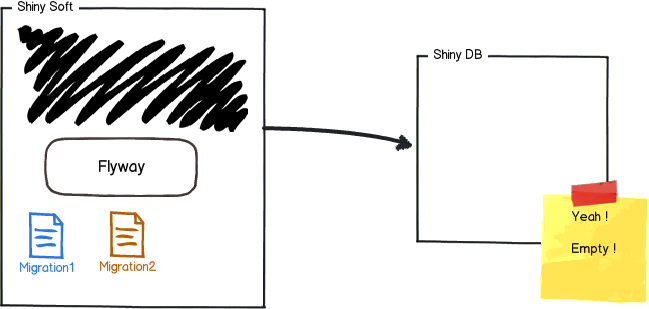
\includegraphics[width=0.45\textwidth]{./chapters/scenarios/images/EmptyDb}
	\caption[Flyway empty database - Source: \cite{FlywayGetStarted}]{Flyway empty database}
	 \label{fig:flyway_empty_db}
\end{figure}
Now the table \textit{flyway\_schema\_history} has been created via the first flyway migration. This metadata table holds various information regarding the database migrations and their history. After this initialization, flyway runs the migration scripts in the sql directory according on their version number subsequently. 
BASELINE MODEL! To start with a baseline

\begin{figure}[H]
	\centering
	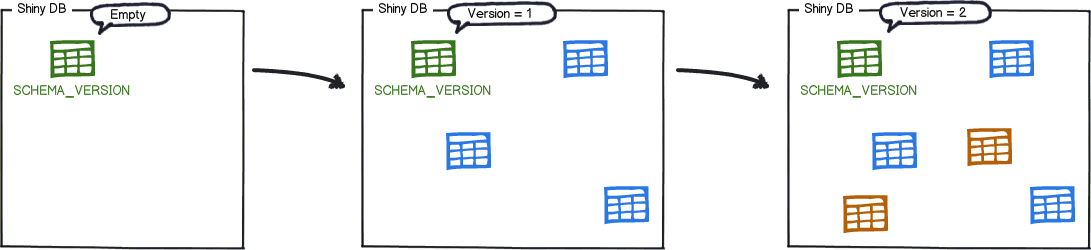
\includegraphics[width=0.85\textwidth]{./chapters/scenarios/images/Migration-1-2}
	\caption[Flyway first migrations - Source: \cite{FlywayGetStarted}]{Flyway first migrations}
	\label{fig:Migration-1-2}
\end{figure}


\marginpar{Rename an attribute}%
The first change specific migration is in the sql migration script\\ \texttt{V3\_\_rename\_attribute.sql}:
\begin{lstlisting}[language=SQL]
ALTER TABLE customer RENAME COLUMN email TO private_email;
\end{lstlisting}
After just adding the script to de sql directory, flyway already knows the change and stores it into the meta data table. With \texttt{flyway info} the migration status can be asked:

\begin{figure}[H]
	\centering
	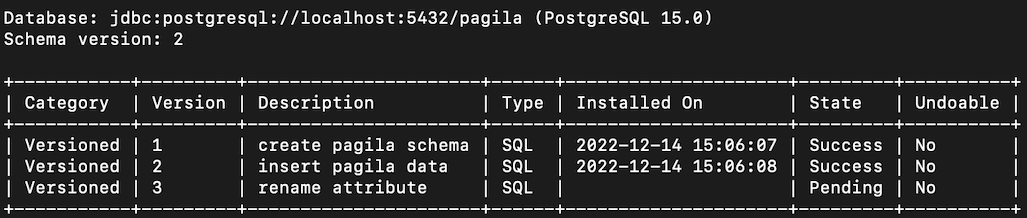
\includegraphics[width=0.95\textwidth]{./chapters/scenarios/images/flyway_metadata_v2}
	\caption[Flyway meta data table - Source: Own illustration]{Flyway meta data table}
	% \label{fig:bsp_chapter:example_figure}
\end{figure}
In order to perform the migration effectively, the command \texttt{flyway migrate} is applied.



\marginpar{Add an\\ attribute}%
To apply the second migration the following script is applied in V3.
\begin{lstlisting}[language=SQL]
ALTER TABLE customer ADD COLUMN gender VARCHAR(50);

UPDATE customer
SET gender = 'undefined';
\end{lstlisting}
Flyway generates a checksum for every applied migration. This checksum is used to track if a file was changes after its applied migration. If such a change occurs, a new migration will cause an error and asks to either revert the change or to run \texttt{flyway repair} to update the schema history.
If a developer would change the default value of gender from \textit{undefined} to \textit{undef} and run a new migration, it would fail. To fix this run \texttt{flyway repair}. Even the environment is now fixed, the change gender equals \textit{undef} is not applied and still \textit{undefined}.


\marginpar{Delete an\\ attribute}%

\begin{lstlisting}[language=SQL]
ALTER TABLE customer
DROP COLUMN gender;
\end{lstlisting}
\todo{chan delete be undoable? Without extra effort.
	How can I undo the deletion? Requires flyway teams.
}

\marginpar{Change an attribute typ}%
To change an attribute type the migration in the file \texttt{V6\_\_change\_attribute\_type.sql} was applied with flyway migrate:
\begin{lstlisting}[language=SQL]
ALTER TABLE customer
ALTER COLUMN private_email TYPE VARCHAR(100) USING private_email::varchar;
\end{lstlisting}


\marginpar{Rename a table and change related view}%
The last migration is to change a related view after renaming a table\\
\texttt{V7\_\_change\_attribute\_type.sql} was applied with flyway migrate:
\begin{lstlisting}[language=SQL]
ALTER TABLE customer RENAME TO clients;
	
	
CREATE OR REPLACE VIEW customer_list AS
SELECT cl.customer_id AS id,
	(cl.first_name || ' '::text) || cl.last_name AS name,
	a.address,
	a.postal_code AS "zip code",
	a.phone,
	city.city,
	country.country,
	CASE
		WHEN cl.activebool THEN 'active'::text
		ELSE ''::text
	END AS notes,
	cl.store_id AS sid
FROM clients cl
JOIN address a ON cl.address_id = a.address_id
JOIN city ON a.city_id = city.city_id
JOIN country ON city.country_id = country.country_id;
\end{lstlisting}

After this last migration the flyway schema history looks like the following:
\begin{figure}[H]
	\centering
	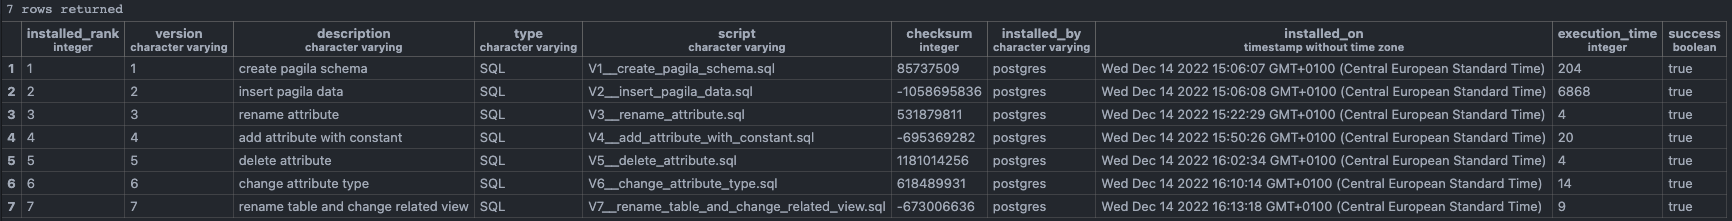
\includegraphics[width=1.1\textwidth]{./chapters/scenarios/images/flyway_schema_history}
	\caption[Flyway Schema History - Source: Own illustration]{Flyway Schema History}
	% \label{fig:bsp_chapter:example_figure}
\end{figure}
For every migration the date inclusive time, the script or the user that applied the script is stored.

\marginpar{Failed migration}%
If a migration fails, an automated rollback is applied.

\subsection{Usage with Java API}
\marginpar{JavaAPI}%
TODO\\



\newpage
\section{Liquibase Scenarios}



\newpage